\chapter{Web Server - Workload Characterization}
L'obiettivo dell'homework è quello di realizzare un workload sintetico semplice e ripetibile, sulla base di un workload reale, attraverso le tecniche descritte nei capitoli precedenti. Successivamente esso deve essere applicato al sistema e, infine, si deve dimostrare che statisticamente si ottiene lo stesso risultato di un workload reale. L'esperimento può essere descritto in tre fasi:
\begin{enumerate}
	\item \textit{Simulazione di un workload reale}. In questa fase si simulano delle richieste random con carico prefissato al sistema. Si collezionano quindi i dati del client (lista delle richieste) di "alto livello" e i dati del server (memoria, utilizzo della CPU, ecc.) di "basso livello". Alla fine di questa fase bisogna analizzare i dati di alto livello per costruire un workload sintetico.
	\item \textit{Applicazione di un workload sintetico}. Dopo aver ricavato il workload sintetico al termine della fase precedente, esso deve essere applicato al sistema. Nuovamente quindi devono essere collezionati i dati di alto livello e basso livello.
	\item \textit{Validazione dei dati}. Prevede un'analisi approfondita dei dati di basso livello del workload reale e sintetico. Essi devono essere oppurtunamente caratterizzati per essere infine confrontati statisticamente. Per farlo si utilizzano dei test statistici meglio descritti successivamente.
\end{enumerate}
Le tre fasi possono essere rappresentate graficamente come nella successiva figura.

\begin{figure}[H]
	\centering
	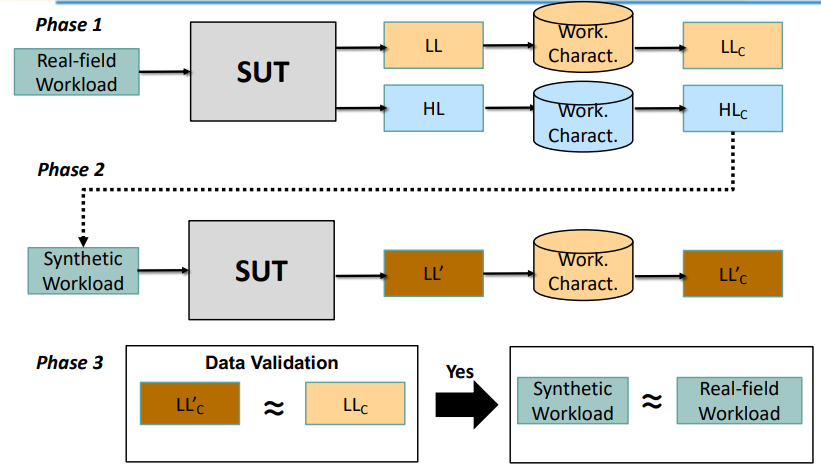
\includegraphics[width=0.6\textwidth]{img/hw3/Overview.png}
	\caption{\textit{Overview WL Characterization}}
\end{figure}

Il server deve essere configurato allo stesso in tutte le fasi. In particolare si è utilizzato lo stesso Web Server descritto nel \textit{Capitolo 2} ma con una diminuzione di prestazioni solo a scopo didattico.

\section{Real-field Workload}
Il primo step prevede di applicare o simulare un workload reale. I dati di alto e basso livello devono essere presi contemporaneamente nel client e nel server.
\subsection{Server}
Il server contiene 10 file di diversa dimensione. I file sono stati scelti tutti dello stesso tipo (file di testo) solo per dimensionarli a piacimento. Nulla vieta però di utilizzare file di tipologie diverse (immagini, documenti, audio, etc.).
\\Essi sono stati dimensionati differenziando i file tra loro di 50 KB e partendo da un minimo di 50 KB. Quindi:
\begin{itemize}
	\item 50k.txt - File di 50 KB
	\item 100k.txt - File di 100 KB
	\item 150k.txt - File di 150 KB	
	\item 200k.txt - File di 200 KB
	\item 250k.txt - File di 250 KB	
	\item 300k.txt - File di 300 KB
	\item 350k.txt - File di 350 KB	
	\item 400k.txt - File di 400 KB	
	\item 450k.txt - File di 450 KB	
	\item 500k.txt - File di 500 KB	
\end{itemize}

\subsubsection{Parametri di basso livello}
Il web server è una macchina virtuale linux. Esistono dunque molti tool in grado di collezionare i parametri caratteristici del sistema. In questo caso è stato utilizzato il tool \textbf{vmstat} (\textbf{Virtual Memory STATistics reporter}) il quale fornisce informazioni circa le performance del sistema su cui viene eseguito. In particolare esse riguardano:
\begin{itemize}
	\item \textbf{Processi}: numero processi in esecuzione o in attesa di essere eseguiti.
	\item \textbf{Memoria}: memoria libera, swap, buffer etc. Ad esempio
		\begin{enumerate}
			\item \textit{free}, quantità di memoria libera.
		\end{enumerate}
	
	\item \textbf{Input/Output}: blocchi ricevuti o inviati da/verso un dispositivo a blocchi.
	\item \textbf{Sistema}: parametri di sistema come ad esempio:
		\begin{enumerate}
			\item \textit{in}, numero di interruzioni al secondo.
			\item \textit{cs}, numero di cambi di contesto al secondo.
		\end{enumerate}
	\item \textbf{CPU}: tipologia di istruzioni che esegue la CPU etc. Ad esempio:
		\begin{enumerate}
			\item \textit{us}, tempo trascorso dalla CPU nell'eseguire codice non-kernel
			\item \textit{sy}, tempo trascorso dalla CPU nell'eseguire codice kernel
			\item \textit{id}, tempo trascorso dalla CPU nello stato di idle
		\end{enumerate}
\end{itemize}
Tali informazioni sono tutte utili ai fini dell'esperimento, ma quelle che evidenziano maggiormente gli effetti della nostra analisi sono quelle relative alla CPU e all'I/O.
\\
Vmstat offre inoltre la funzionalità di eseguire un campionamento dei parametri ad una frequenza e durata prefissata, tramite l'apposito comando eseguibile da terminale:
\begin{minted}[framesep = 1mm,
	fontsize = \footnotesize,
	breaklines,
	]{PYTHON}
	vmstat -n 1 400
\end{minted}
Il primo parametro "1" indica il periodo di campionamento in secondi, mentre il secondo parametro "400" indica la durata totale di esecuzione in secondi. L'output poi può essere semplicemente salvato in un file di testo o csv.
\\
Tale comando è stato avviato pochi secondi prima dell'avvio del test su JMeter, ed ha continuato a campionare per qualche secondo anche dopo la sua fine, dunque nell'analisi dei dati sono attesi parametri il cui andamento evidenzia le varie fasi.


\subsection{Client - JMeter}
La simulazione degli utenti che fanno accesso al server è stata possibile tramite il tool JMeter, già descritto nei capitoli precedenti. 
\\In particolare sono stati realizzati tre Thread Group ognuno composto da 10 Thread (l'equivalente di 10 utenti) con una durata di simulazione pari a 2 min ciascuno. Ogni gruppo contiene 10 richieste riferite alle 10 risorse disponibili nel web server. Esse vengono poi eseguite in modo casuale tramite un apposito controller. 
\begin{figure}[H]
	\centering
	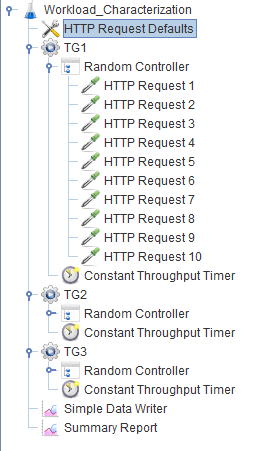
\includegraphics[width=0.4\textwidth]{img/hw3/jmeter_reale.png}
	\caption{\textit{Configurazione di JMeter per la simulazione di un workload reale}}
\end{figure}
Ogni gruppo inoltre ha un suo specifico carico. In questo caso si ha:
\begin{itemize}
	\item \textbf{TG1} : 400 richieste al minuto
	\item \textbf{TG2} : 550 richieste al minuto
	\item \textbf{TG3} : 700 richieste al minuto
\end{itemize}
Essi vengono poi eseguiti in sequenza e non in parallelo. Questo perché si possono creare possibili conflitti sulle risorse, dati dal fatto che ogni gruppo richiede le stesse risorse degli altri. 
\subsubsection{Parametri di alto livello}
I parametri di alto livello possono essere collezionati direttamente tramite il tool JMeter e salvati in formato \textit{.cvs}. Non sono necessari dunque programmi esterni. I parametri utili ai fini dell'analisi sono:
\begin{itemize}
	\item \textbf{Timestamp}, l'istante di tempo in cui viene effettuata la corrispettiva richiesta (in millisecondi)
	\item \textbf{elapse}, inteso come Response Time
	\item \textbf{label}, contiene l'informazione categorica della richiesta effettuata.
	\item \textbf{bytes}, numero di byte ricevuti tramite la relativa richiesta.
	\item \textbf{sentBytes}, numero di byte inviati per effettuare la richiesta.
	\item \textbf{latency}
	\item \textbf{connect}, tempo di connessione misurato per effettuare l'handshake TCP (in millisecondi).
\end{itemize}

\subsection{Workload Characterization}
Le misure vengono effettuate correttamente avviando prima \textit{vmstat} nel server e in seguito JMeter sul client in modo che i dati vengono salvati contemporaneamente nel lato client (alto livello) e nel lato server (basso livello). Al termine della simulazione quindi ci si ritrovano due file di dati.

\subsubsection{Parametri di alto livello}
I parametri di alto livello vanno incontro alla procedura di filtraggio, PCA e Clustering per ridurne la dimensionalità.
\\Essi appaiono nel seguente modo:
\begin{figure}[H]
	\centering
	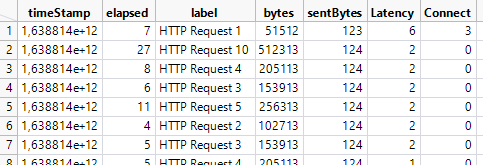
\includegraphics[width=0.8\textwidth]{img/hw3/alto_livello_esempio.png}
	\caption{\textit{Parametri di alto livello utili ai fini dell'analisi}}
\end{figure}
\hrule
\vspace{0.3cm}
La fase di filtraggio non prevede nessuna azione di modifica del dataset.
\\Sul dataset originale quindi deve essere effettuata la PCA per cercare di ridurne la dimensionalità senza perdere troppa varianza. Bisogna soprattutto considerare che per questi parametri la fase di Clustering è molto importante poiché racchiude le informazioni principali per costruire il workload sintetico.
\vspace{0.3cm}
\hrule
\vspace{0.3cm}
Tramite la PCA sono state scelte tutte le componenti principali, mantenendo una varianza del 100\%.
\begin{figure}[H]
	\centering
	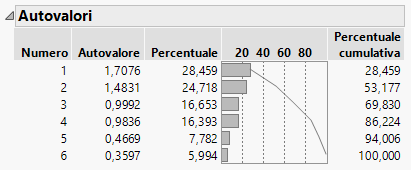
\includegraphics[width=0.6\textwidth]{img/hw3/autovalori.png}
	\caption{\textit{Analisi della varianza tramite autovalori}}
\end{figure}
Sulla base di queste può essere effettuato il clustering gerarchico.
\vspace{0.3cm}
\hrule
\vspace{0.3cm}
Il numero di cluster rappresenta il numero di richieste del workload sintetico, poiché in ogni cluster viene scelto un elemento rappresentativo di esso stesso. A tal proposito quindi il numero di cluster non deve essere maggiore del numero di \textit{HTTP Request} totali utilizzate durante la simulazione (in questo caso 30) e non deve essere un numero molto elevato. Al tempo stesso però non si deve perdere molta varianza a causa della clusterizzazione. 
\\La via più semplice è quella di effettuare delle prove scegliendo un numero di cluster minore della metà (in questo caso minore di 15) e valutare per ogni numero quanta varianza si perde.
\\Partendo da 6 componenti principali si può scegliere un numero di cluster variabile e calcolare la devianza persa per ogni valore.
\begin{center}
	\begin{tabular}{|c|c|c|c|c|c|}
		\hline
		\textbf{6 Cluster} & \textbf{8 Cluster} & \textbf{10 Cluster} &\textbf{12 Cluster} \\
		\hline
		35\% & 27\%& 21.5\% & 17\% \\
		\hline
	\end{tabular}
\end{center}
La scelta ricade su 10 cluster in modo da avere un workload sintetico abbastanza ristretto e una perdita di varianza non troppo elevata.
\\Per scegliere gli elementi rappresentativi di un cluster si può ricorrere a vari metodi:
\begin{itemize}
	\item Il punto più centrale possibile
	\item Il punto in cui un valore categorico si ripete più volte. Applicabile però solo se il dataset ha un parametro categorico in un insieme limitato di valori.
	\item Casualmente
	\item Il punto che si avvicina il più possibile alla media del cluster
	\item Etc.
\end{itemize}

\subsubsection{Parametri di basso livello}
\begin{figure}[H]
	\centering
	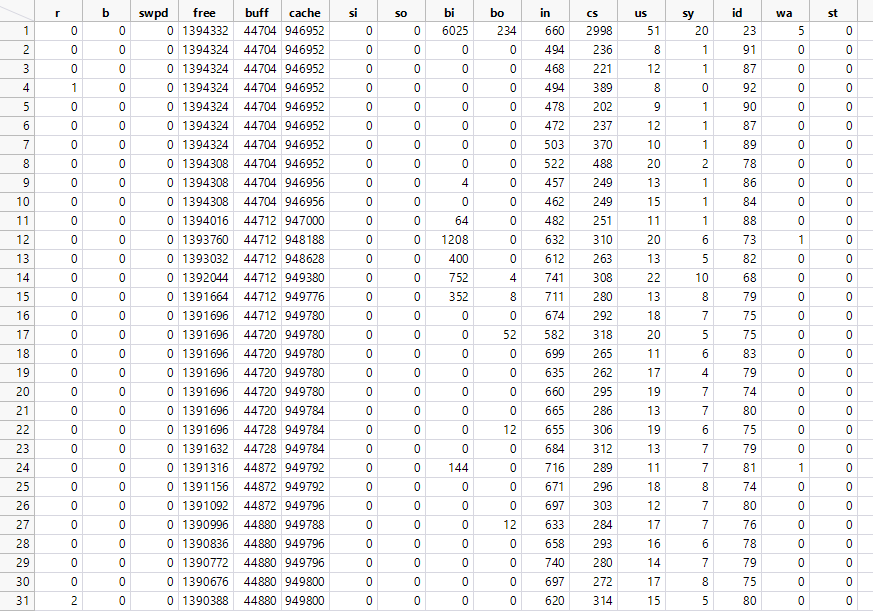
\includegraphics[width=0.7\textwidth]{img/hw3/porzione_lowlevel.png}
	\caption{\textit{Porzione dataset - Low Level Parameters}}
\end{figure}
I parametri di basso livello costituiscono un dataset formato da 17 colonne e 400 righe. Su di esso sono state dunque effettuate operazioni di \textit{filtraggio}, \textit{PCA} e \textit{clustering}, procedendo in maniera analoga a quanto già si era fatto nel Capitolo 1.
\\
\hrule
\vspace{0.3cm}
Analizzando le distribuzioni sono state individuate 4 colonne costanti (e quindi da rimuovere): \textbf{swpd}, \textbf{si}, \textbf{so}, \textbf{st}.
\\
Dopodichè sono state eliminate tutte le righe associate ai campioni prelevati da vmstat quando il client non stava sottoponendo richieste al server, in quanto non forniscono informazioni utili agli scopi della caratterizzazione.
\\
Per fare ciò sono stati analizzati gli andamenti in funzione del tempo dei parametri relativi all'utilizzo della CPU precedentemente descritti.
\begin{figure}[H]
	\subfigure{	
		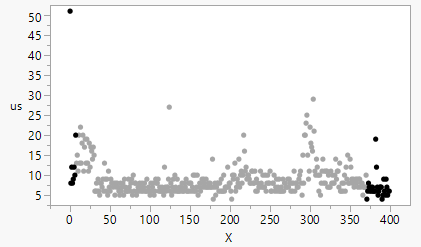
\includegraphics[width=0.30\textwidth]{img/hw3/us.png}}
	\subfigure{	
		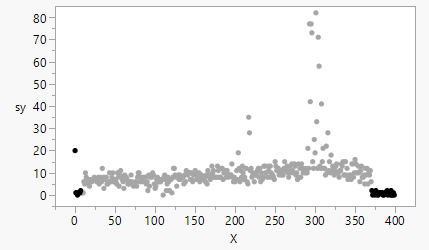
\includegraphics[width=0.30\textwidth]{img/hw3/sy.png}}
	\subfigure{	
		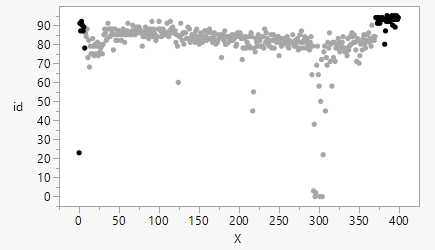
\includegraphics[width=0.30\textwidth]{img/hw3/id.png}}
	\caption{\textit{Andamento parametri CPU}}
\end{figure}
In particolare, osservando i grafici di \textit{sy} e \textit{id} risultano evidenti queste "fasi" nelle quali il processore trascorre meno tempo ad eseguire codice kernel e più tempo in idle rispetto a quando si sta sottoponendo il workload, visto che non è impegnato nel servire le richieste.
\\
Discorso analogo lo si può fare osservando le interruzioni al secondo (\textbf{in}), che incrementano drasticamente nel corso della recezione delle richieste, per poi diminuire in queste fasi.
\begin{figure}[H]
	\centering   
	\subfigure{	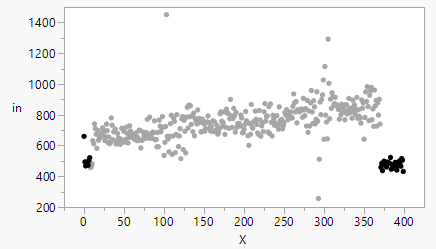
\includegraphics[width=0.30\textwidth]{img/hw3/interrupts.png}}
	\subfigure{
		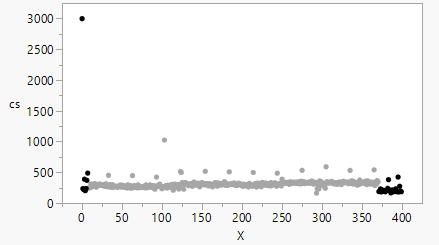
\includegraphics[width=0.30\textwidth]{img/hw3/cs1.png}}
	\caption{\textit{Andamento parametri di Sistema e CPU}}
\end{figure}
Contestualmente è stata eliminata anche la prima riga (outlier per quasi tutti i parametri), in quando è stata associata alla fase di avvio dell'esecuzione del comando vmstat e quindi non di particolare interesse per gli scopi dell'esperimento.
\\
L'ultima operazione effettuata in questa prima fase di filtraggio è stata la rimozione di un outlier associato al parametro \textbf{b}, il quale è indice del numero di processi sospesi ed in attesa di risorse per poter essere riattivati.
Essendo outlier anche di \textbf{wa} (tempo trascorso dalla CPU in attesa di input/output) è quasi sicuramente indice dello stesso fenomeno, il quale è stato da noi considerato come casuale e quindi trascurabile.
\begin{figure}[H]
	\centering
	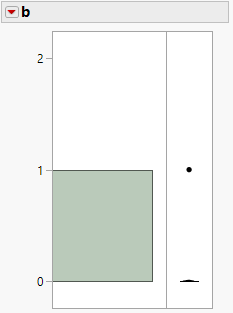
\includegraphics[width=0.3\textwidth]{img/hw3/outlaier_b.png}
	\caption{\textit{Distribuzione di b}}
\end{figure}
La riga ad esso associata è la 122, la quale è stata opportunamente rimossa. A seguito di questa cancellazione, la colonna associata al parametro b è diventata costante ed è dunque stata eliminata.
\\
Il dataset ottenuto è formato da 12 colonne e circa 360 righe. Il numero di righe risultante può essere ulteriormente validato se consideriamo che la durata del test è proprio di 360 secondi.
\vspace{0.3cm}
\hrule
\vspace{0.3cm}
Su questi dati è stata effettuata la PCA, a seguito della quale sono state prese in considerazione \textit{7 componenti principali}, le quali spiegano il 92,768 \% della devianza totale.
\begin{figure}[H]
	\centering
	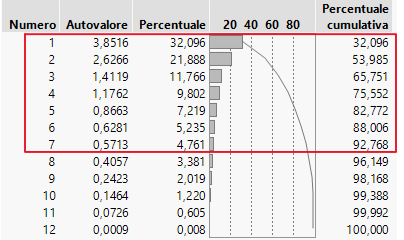
\includegraphics[width=0.5\textwidth]{img/hw3/PCA7.png}
	\caption{\textit{PCA Low-Level Filtered}}
\end{figure}
\hrule
\vspace{0.3cm}
Per non perdere una porzione significativa di devianza, dopo vari test, si è deciso di selezionare \textbf{20 Cluster} conservandone il 78,36\%.
\\
Infine è stata implementata in Matlab la seguente funzione per scegliere l'elemento rappresentativo di ogni cluster:
\begin{minted}[framesep = 1mm,
	fontsize = \footnotesize,
	breaklines,
	]{MATLAB}
	function [new_workload] = random_selection(workload)
	%workload = colonne PCA + colonna cluster
	N_cluster = max(workload(:,end)); %numero cluster
	[r,c] = size(workload);
	
	%isolo la colonna dei cluster
	cluster_data = workload(:,end);
	
	new_workload = zeros(N_cluster,c);
	
	%itero per ogni cluster
	for i = 1:N_cluster
	%prelevo tutti gli indici di riga associati ad uno stesso cluster i
		index = find(cluster_data==i); 
		%se ho più di una riga ne scelgo una random
		if length(index) > 1
			new_workload(i,:) = workload(randsample(index,1),:); 
		else
			%se ho solo una riga scelgo quella
			new_workload(i,:) = workload(index,:);
		end
	end
	end
\end{minted}
La funzione riceve in input le colonne estratte dalla PCA affiancate alla colonna dei cluster, la quale specifica il cluster di appartenenza di ciascuna riga.
Come si evince dal codice, i centroidi sono stati selezionati in maniera randomica nel caso in cui nel cluster sia presente più di un elemento.
\\
L'output della funzione è un workload costituito da 7 colonne e 20 righe, rappresentativo di quello originario.

\section{Synthetic Workload}
A partire dalla clusterizzazione di alto livello, identificati gli elementi rappresentativi di ogni cluster, si deve rifare la simulazione ma con il workload sintetico.
\\Il dataset in esame è composto da un parametro categorico che rappresenta la richiesta effettuata (risorsa e utente) facendo parte di un insieme molto limitato. La scelta dell'elemento rappresentativo può ricadere nel scegliere la \textit{label} che si ripete in più punti nello stesso cluster.
\\A tal proposito si può calcolare una tabella che per ogni cluster indica il numero di ricorrenze del valore del parametro categorico.
\begin{figure}[H]
	\centering
	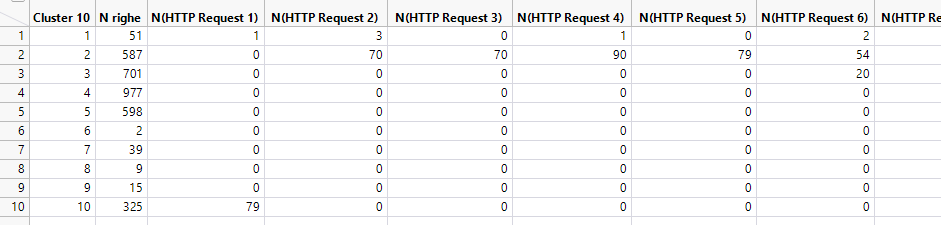
\includegraphics[width=\textwidth]{img/hw3/cluster_label.png}
	\caption{\textit{Tabella che associa ad ogni cluster il numero di punti con una determinata \textit{label}}}
\end{figure}
La matrice che compone la tabella è una matrice 10x30 (10 cluster e 30 richieste possibili) e bisogna calcolare il massimo di riga per ogni riga. Inoltre se il massimo di riga è associato ad una \textit{label} già selezionata in precedenza, allora si deve scegliere il secondo massimo nella riga e così via. Si può automatizzare il tutto tramite uno script MATLAB:
\begin{minted}[framesep = 1mm,
	fontsize = \footnotesize,
	breaklines,
	]{MATLAB}
%% Dati
[data, txt] = xlsread('label-cluster 10');
data_filter = data(:, 3:end); 
txt_filter = txt(:, 3:end)';

%% Ricerca centroidi
[r,c] = size(data_filter);
max_list = zeros(1,r);  % Lista dei massimi
max_index = zeros(1,r); % Lista degli indici dei massimi

%Inizializzo vettore degli indici
for i=1:r
	max_index(i) = -1;
end

for i=1:r
	[temp_v, temp_i] =  max(data_filter(i,:));
	while ismember(temp_i,max_index)
		data_filter(i,temp_i) = -1;
		[temp_v, temp_i] =  max(data_filter(i,:));
	end
	max_list(i) = temp_v;
	max_index(i) = temp_i;
end

%% Stampa risultati
sort(txt_filter(max_index))
\end{minted}
Il risultato dello script è la lista delle \textit{label} che identificano il workload sintetico.
\begin{enumerate}
	\item HTTP Request 1 :  TG1 con risorsa \textit{200k.txt}
	\item HTTP Request 11 : TG2 con risorsa \textit{50k.txt}
	\item HTTP Request 17 : TG2 con risorsa \textit{350k.txt}
	\item HTTP Request 21 : TG3 con risorsa \textit{50k.txt}	
	\item HTTP Request 22 : TG3 con risorsa \textit{100k.txt}		
	\item HTTP Request 23 : TG3 con risorsa \textit{150k.txt}		
	\item HTTP Request 25 : TG3 con risorsa \textit{250k.txt}		
	\item HTTP Request 27 : TG3 con risorsa \textit{350k.txt}
	\item HTTP Request 28 : TG3 con risorsa \textit{400k.txt}			
	\item HTTP Request 29 : TG3 con risorsa \textit{450k.txt}		
\end{enumerate}

\subsection{Server}
Il server non deve essere assolutamente modificato. Tutte le configurazioni effettuate per il workload reale rimangono invariate

\subsubsection{Parametri di basso livello}
I parametri di basso livello devono essere collezionati allo stesso modo utilizzato nel workload reale. Essi devono essere confrontati con i parametri di basso livello salvati durante la simulazione del workload reale. Questa operazione verrà analizzata nel paragrafo \textit{Data Validation}.

\subsection{Client - JMeter}
Il client deve, a questo punto, simulare le nuove richieste applicando il workload sintetico ricavato con l'analisi. Anche in questo caso la configurazione di JMeter non deve essere modificata, tranne che per le richieste.
\begin{figure}[H]
	\centering
	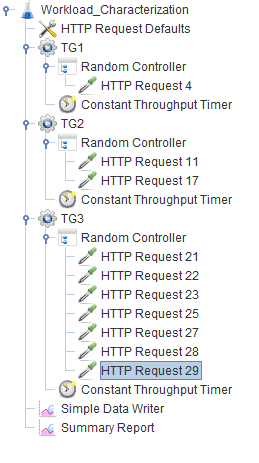
\includegraphics[width=0.4\textwidth]{img/hw3/jmeter_sintetico.png}
	\caption{\textit{Configurazione di JMeter per il workload sintetico}}
\end{figure}

\subsubsection{Parametri di alto livello}
I parametri di alto livello possono anche non essere collezionati poiché non servono per ulteriori analisi. Per completezza però si possono salvare tramite lo stesso JMeter usato per la simulazione.


\subsection{Workload Characterization}
La caratterizzazione può essere applicata solo ai parametri di basso livello. Il risultato viene confrontato con la caratterizzazione degli stessi parametri misurati con il workload reale. Deve necessariamente accadere che il numero di colonne di questi parametri sia lo stesso.
\subsubsection{Parametri di basso livello}
Anche in questo caso il dataset di basso livello è costituito da 17 colonne e 400 righe. Analogamente a quanto fatto in precedenza per i parametri relativi al Workload reale sono state eseguite le operazioni di filtraggio, PCA e clustering.
\\
Sono state eliminate le colonne costanti, che in questo caso sono: \textbf{b}, \textbf{swpd}, \textbf{si}, \textbf{so} e \textbf{st}.
\\
Dopodichè, eliminando le righe relative ai campionamenti nelle fasi in cui il sistema non stava servendo alcuna richiesta, il set di dati è stato ulteriormente ridotto. L'analisi degli outlier non ha portato all'eliminazione di alcuna riga, in quanto tutti i punti oltre i quartili dei box-plot sono stati considerati significativi. 
\\
\hrule
\vspace{0.3cm}
Come accaduto anche in precedenza, il dataset risultate è composto da 12 colonne e circa 360 righe (coerentemente con il tempo di sottomissione del workload).
\\
\begin{figure}[H]
	\centering
	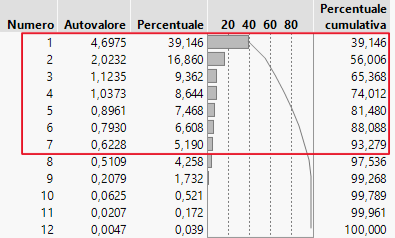
\includegraphics[width=0.5\textwidth]{img/hw3/PCA7_syn.png}
	\caption{\textit{PCA syn Low-Level Filtered}}
\end{figure}
Per la PCA è stato scelto lo stesso numero di componenti selezionate nella caratterizzazione dei parametri di basso livello del workload reale.
Questa è stata una scelta obbligata dal fatto che le funzioni Matlab utilizzate per la validazione operano su matrici le quali devono necessariamente avere lo stesso numero di colonne.
\\
In ogni caso selezionando tali componenti si riesce a mantenere un'ottima percentuale di devianza: il 93,279\%.
\\
\hrule
\vspace{0.3cm}
Anche qui la scelta più conveniente in termini di devianza persa è stata quella di suddividere il dataset in 20 Cluster, conservandone il 75,51\% della totale. 
\\
Infine il workload di basso livello così ottenuto, è stato dato in input alla funzione \textit{random\_selection}, già descritta in precedenza, per ricavare i centroidi di ogni cluster.
\section{Data Validation}
I parametri di basso livello relativi a workload reale e sintetico, ottenuti in seguito alla caratterizzazione sono i seguenti:
\begin{figure}[H]
	\centering
	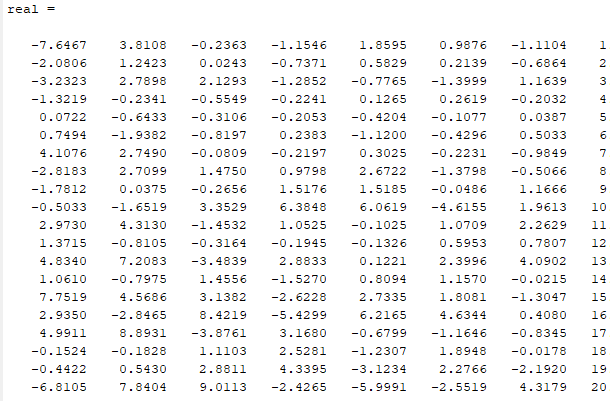
\includegraphics[width=0.6\textwidth]{img/hw3/real_wl.png}
	\caption{\textit{Low-Level Parameters Real WL}}
	\label{real}
\end{figure}
\begin{figure}[H]
	\centering
	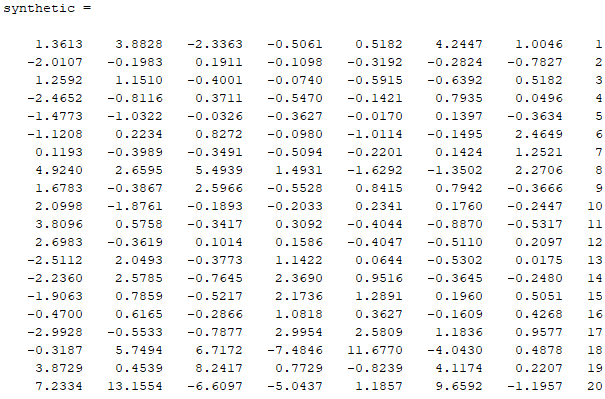
\includegraphics[width=0.6\textwidth]{img/hw3/syn_wl.png}
	\caption{\textit{Low-Level Parameters Synthetic WL}}
	\label{syn}
\end{figure}
Sono questi che andranno statisticamente confrontati per validare il Workload Sintetico.
\\La procedura per la validazione è molto semplice:
\begin{enumerate}
	\item Normalità verificata. Se i due dataset provengono da una distribuzione normale allora si possono eseguire test parametrici per la validazione. In particolare si possono usare vari tipi di test statistici anche in base all'omoschedasticità dei campioni.
	\begin{enumerate}
		\item Omoschedasticità verificata. Se i due dataset sono omoschedastici allora si possono utilizzare test sulla base di questa condizione verificata.
		\item Omoschedasticità non verificata. Se i due dataset non rispettano la proprietà di omoschedasticità allora bisogna utilizzare test che si basano su tale condizione non verificata.
	\end{enumerate}
	\item Nomarlità non verificata. Se i due dataset non provengono da una distribuzione normale allora si devono usare necessariamente test statistici non parametrici per la validazione.
\end{enumerate}

\subsection{Normalità}
Per verificare se un campione proviene da una popolazione con distribuzione normale, ci si può affidare a test visivi oppure a test statistici analitici.
\subsubsection{Test Visivo}
Visivamente si può capire se un campione proviene da una popolazione con distribuzione normale effettuando un grafico dei quantili del campione rispetto ai quantili di una distribuzione normale. Ciò lo si realizza sfruttando la funzione Matlab \textbf{qqplot}.
\\Ad esempio prendendo una componente principale del workload reale (dopo la caratterizzazione) si può effettuare un grafico dei quantili:
\begin{figure}[H]
	\centering
	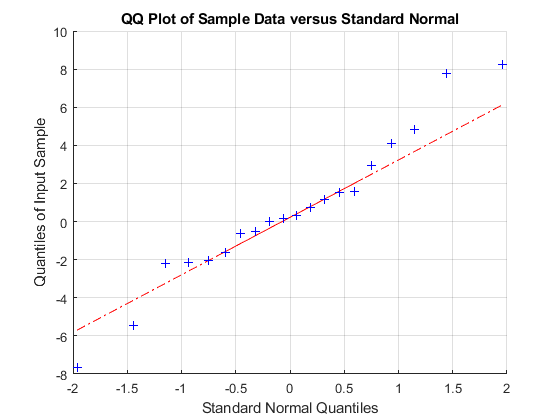
\includegraphics[width=0.8\textwidth]{img/hw3/test_visivo.png}
	\caption{\textit{Grafico Quantili-Quantili della prima componente principale del workload reale caratterizzato}}
\end{figure}
Come si può notare il campione non proviene da una distribuzione normale.
\subsubsection{Test analitico}
Un test analitico è il test di \textbf{Kolmogorov-Smirnov}. Esso si basa sull'ipotesi nulla $H_0$:
\begin{equation*}
	H_0 : N(0,1) 
\end{equation*}
ovvero che i dati in input provengono da una distribuzione normale standard.
\\In MATLAB esiste una funzione già definita per eseguire questo tipo di test: \textbf{[h,p] = kstest(x)}. Esso fornisce in output il risultato del test (se $H_0$ viene rigettata o meno) con il relativo \textit{P-Value}. In particolare \textit{h} è 1 se il test rigetta l'ipotesi nulla $H_0$ con un livello di significatività del 5\%, 0 altrimenti.
\subsubsection{Caso di studio - Implementazione}
Per la verifica della normalità si sono quindi applicate queste funzioni ai dataset (Fig.\ref{real} e Fig.\ref{syn}).
\begin{minted}[framesep = 1mm,
	fontsize = \footnotesize,
	breaklines,
	]{MATLAB}
	%% Data
	real1 = xlsread('real');
	synthetic1 = xlsread('syn');
	
	real = random_selection(real1);
	synthetic = random_selection(synthetic1);
	
	N = size(real,2); %numero di colonne lo stesso per i due set di dati
	real = real(:, 1:N-1); % rimuovo la colonna associata ai cluster
	synthetic = synthetic(:, 1:N-1); % lo stesso
	
	%verifica Normal Distribution kstest
	[h_ks_real, p_ks_real] = kstest(real);
	[h_ks_syn, p_ks_syn] = kstest(synthetic);
	
	%verifica Normal Distribution visual test
	figure();
	subplot(2,1,1);
	qqplot(real);
	subplot(2,1,2);
	qqplot(synthetic);
\end{minted}
L'output della kstest è 1 per entrambi i workload, quindi entrambi non provengono da una distribuzione normale. Per completezza si riportano i grafici del quantile-quantile plot associato ad ogni PC dei dataset, i quali confermano il risultato del test di Kolmogorov-Smirnov.
\begin{figure}[H]
	\centering
	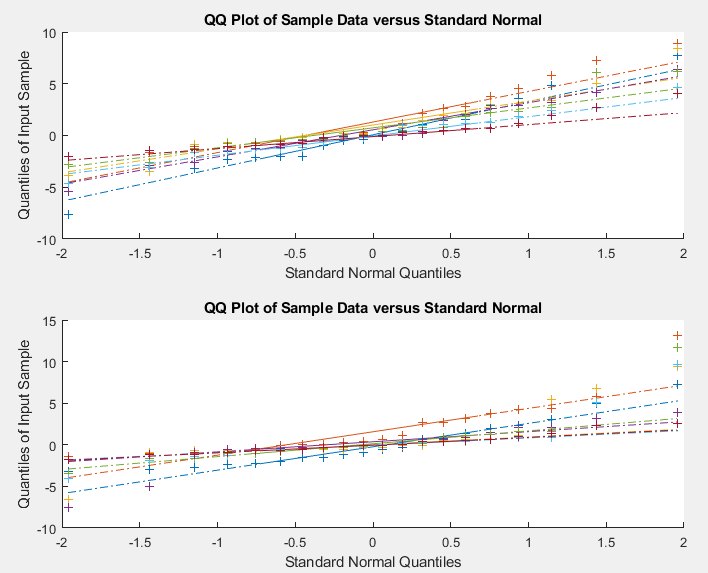
\includegraphics[width=0.5\textwidth]{img/hw3/qqplot.png}
	\caption{\textit{quantile-quantile plot di Fig.\ref{real} e Fig.\ref{syn}}}
\end{figure}
Ciò suggerisce l'utilizzo di test non parametrici per la validazione.
\subsection{Omoschedasticità}
Anche se nel caso di studio la verifica dell'omoschedasticità non è richiesta, visto che entrambi i set di dati non provengono da una distribuzione normale, per completezza ne riportiamo il procedimento.
\\
Tale proprietà è verificata nel momento in cui diversi campioni hanno stessa varianza (non è detto che essa sia nota), anche se provengono da popolazioni (distribuzioni) differenti. Questa è una caratteristica necessaria da verificare prima di applicare i test parametrici, ad esempio. Difatti, eseguire un test senza aver effettuato questo controllo può avere un impatto significativo sui suoi risultati, fino ad invalidarli.
\subsubsection{Test Visivo}
Visivamente possiamo capire se le varianze delle due distribuzioni sono simili, tramite il \textbf{boxplot}. All'aumentare della lunghezza del box aumenta la varianza dei dati che "rappresenta".
\begin{figure}[H]
	\centering
	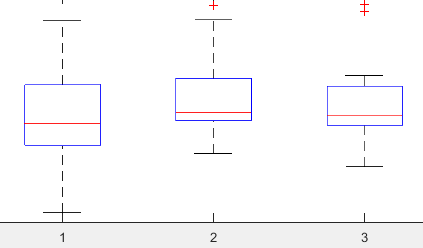
\includegraphics[width=0.5\textwidth]{img/hw3/boxplot.png}
	\caption{\textit{boxplot I,II e III componente del WL reale}}
\end{figure}
\subsubsection{Test analitico}
Un test analitico per il check sull'uguaglianza delle varianze dei campioni è: 
\\
\textbf{h = vartest2(x,y)}.
\\
Esso è applicabile esclusivamente se i due campioni provengono da una distribuzione normale.
Si basa sull'ipotesi nulla $H_0$:
\begin{enumerate}
	\item $H_0$ : i vettori x ed y provengono da distribuzioni normali e con uguale varianza. 
\end{enumerate}
Il suo output h è 1 se il test rigetta l'ipotesi nulla $H_0$ con un livello di significatività del 5\%, 0 altrimenti.
\subsection{Validazione}
Per completezza è riportato l'intero script, nel quale è stato previsto anche il caso in cui i campioni provengono da distribuzioni normali.
\\
\begin{minted}[framesep = 1mm,
	fontsize = \footnotesize,
	breaklines,
	]{MATLAB}
	%se almeno una delle due distribuzioni non è normale
	%applico il test non parametrico
	if ((h_ks_real | h_ks_syn) == 1)   
	[p_wilc,h_wilc] = NoParametric(real,synthetic,N);
	else
	%distribuzioni normali (risultato di quell if è 0)
	%check sulle varianze
	[h_var, p_var] = vartest2(synthetic, real);
	
		%se le due distribuzioni hanno stessa varianza
		if (h_var == 0)
		%applico il two sample t-test
		[h_ttest, p_ttest] = ttest2(syntetic, real);
		else
		%se le due distribuzioni non hanno stessa varianza
		[h_ttest_novar, p_ttest_novar] = ttest2(syntetic, real, 'Vartype', 'unequal');
		end
	
	end
\end{minted}
Come già detto precedentemente, i nostri campioni soddisfano la condizione del primo \textit{if} quindi viene eseguita la funzione \textit{NoParametric}:
\begin{minted}[framesep = 1mm,
	fontsize = \footnotesize,
	breaklines,
	]{MATLAB}
	function [p_wilc,h_wilc] = NoParametric(real,synthetic,N)
		p_wilc = zeros(1,N-1);
		h_wilc = zeros(1,N-1);
		for i = 1:N-1
			[p_wilc(i),h_wilc(i)] = 
			ranksum(synthetic(:,i), real(:,i));
		end
	end
\end{minted}
Essa richiama la funzione MATLAB 
\\
\textbf{[p,h] = ranksum(x,y)}
la quale esegue il test non parametrico di \textbf{Wilcoxon}. Esso si basa sull'ipotesi nulla $H_0$:
\begin{enumerate}
	\item $H_0$ : i dati di x ed y provengono da distribuzioni continue con uguale mediana. 
\end{enumerate}
Tale funzione opera sulle singole colonne delle matrici x ed y e quindi bisogna iterare il procedimento per il numero di colonne.
Se l'output h è uguale ad 0, si ha un fallimento nel rigettare l'ipotesi nulla con un livello di significatività del 5 \%, il contrario se è 1.
\\
L'output di \textit{NoParametric} sarà dunque costituito da due vettori:
\begin{enumerate}
	\item p\_wilc : il vettore degli p-value per ogni componente principale.
	\item h\_wilc : il risultato della ranksum su ogni componente principale di x ed y. 
\end{enumerate}
L' \textbf{h\_wilc} calcolata sui campioni sotto studio è un vettore di tutti zeri:
\begin{figure}[H]
	\centering
	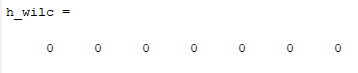
\includegraphics[width=0.5\textwidth]{img/hw3/h_wilc.png}
	\caption{\textit{output test di Wilcoxon}}
\end{figure}
ciò significa che l'ipotesi nulla non è stata rigettata per ogni componente principale e che quindi Workload Reale e Workload Sintetico hanno determinato effetti statisticamente simili sul server.
\\
\textbf{Il Workload Sintetico ottenuto è una buona approssimazione di quello Reale}.